\documentclass[11pt, oneside]{article}   	% use "amsart" instead of "article" for AMSLaTeX format
\usepackage[margin=0.7in]{geometry}                		% See geometry.pdf to learn the layout options. There are lots.
\geometry{letterpaper}                   		% ... or a4paper or a5paper or ... 
%\geometry{landscape}                		% Activate for rotated page geometry
%\usepackage[parfill]{parskip}    		% Activate to begin paragraphs with an empty line rather than an indent
\usepackage{graphicx}				% Use pdf, png, jpg, or eps§ with pdflatex; use eps in DVI mode
								% TeX will automatically convert eps --> pdf in pdflatex		
\usepackage{amssymb}
\usepackage{amsmath}
\usepackage{amsfonts}
\usepackage{listings}
\usepackage{dsfont}

%SetFonts

%SetFonts


\title{Sensitivity of Oxide ABR Transient Response with $\tau$}
\author{Chris Keckler}
%\date{}							% Activate to display a given date or no date

\begin{document}
\maketitle

After the optimal ARC design for the 1000 MWth oxide-fuelled ABR was chosen through parametric analysis to have $w = \$0.87$, $S = 65$ C, and $\Delta T_{act} = 10$ C (see \cite{2017ANSWinter_ARC}), the sensitivity of the design to the ARC heat transfer constant, $\tau$, was examined.
Through COMSOL multiphysics finite element simulations, the time constant for heat transfer from the primary coolant to the ARC upper reservoir fluid was optimized down to 1.3 s \cite{1stARC_paper}.
This is accomplished through the use of an annular upper reservoir designed specifically for the fuel assembly present in ABR cores. 
Using $\tau=1.3$ s, it was determined that no oscillations are induced into the system response to the ULOHS, UTOP, and ULOF transient scenarios. 
The purpose of this study was to determine if the transient response utilizing the optimal ARC design is particularly sensitive to the $\tau$ parameter. 
This was done by modifying the input decks for the three transients to have longer time constants in 0.5 s increments from 1.3 s up through 4.8 s -- nearly a 4x increase.
The results of this sensitivity study for the three transients are presented below.

%%%%%%%%%%%%%%%%%%%%%%%%%%%%%%%%%%%%%%%%%%%%%%%%%%%%%%%%%%%%%%%%%%%%%%%
\section{ULOHS}
Figure \ref{fig:ULOHS_peak} shows the peak coolant temperatures with time of each ULOHS simulation for all $\tau$ values on a single plot. 
Because each simulation gives very nearly the same values throughout the transient for all values of $\tau$, it is difficult to distinguish between the different cases. 
Similarly, Figure \ref{fig:ULOHS_rho} shows both the reactivity introduced from the ARC system as well as the net reactivity throughout the ULOHS transient for all values of $\tau$. 
Again, virtually no difference is seen between the different SAS runs, and the lines essentially completely overlap. 
Even when $\tau$ is brought up to 20 s (not depicted), the difference in transient performance is minimal.
No instabilities are formed - rather the temperature and ARC reactivity behavior is simply shifted by about 15 seconds in the transient phase of the simulation, but the maximum and asymptotic temperatures remain the same.
These results indicate that the ULOHS scenario with the optimal ARC system implemented is very insensitive to the heat transfer time lag between coolant and ARC reservoir.
This favorable behavior is likely due to the monotonicity and smoothness of temperature and reactivity changes in a ULOHS scenario.

\begin{figure}[h!]
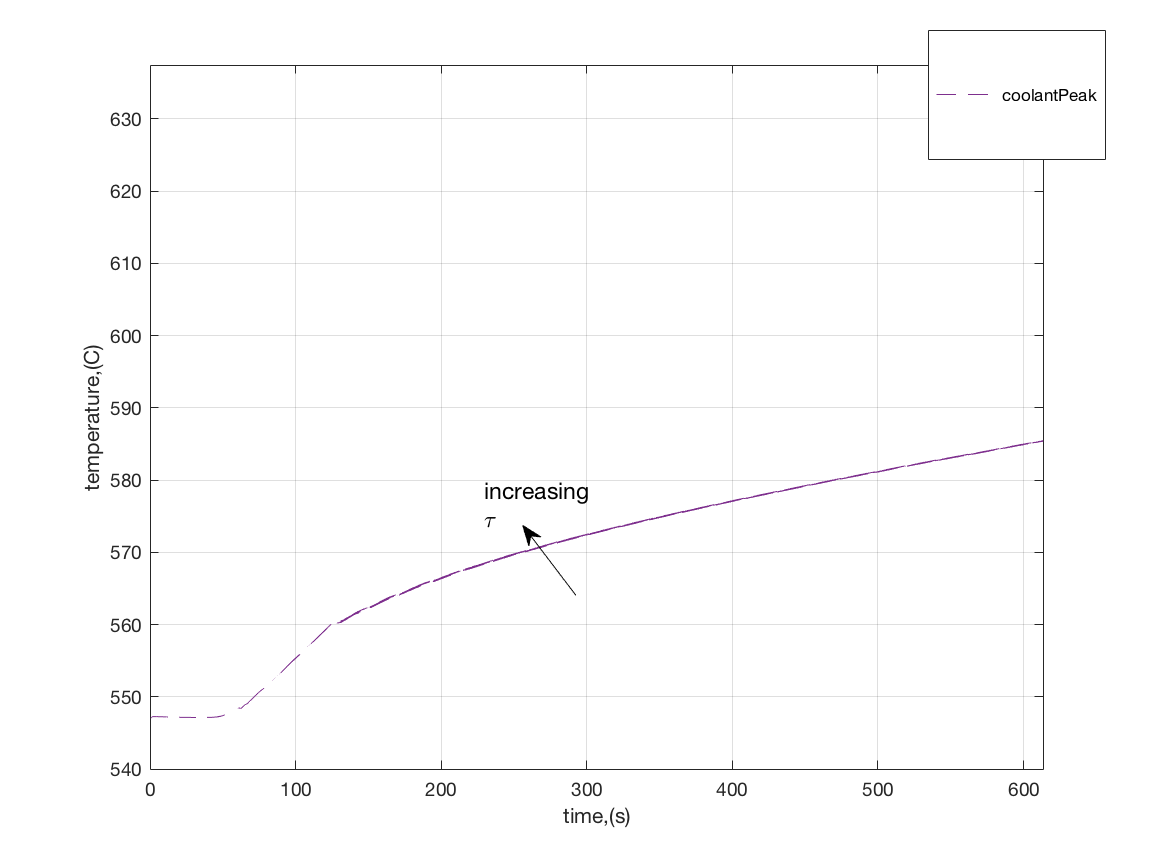
\includegraphics[width=10cm]{ULOHS_peak}
\centering
\caption{Peak coolant temperature in the oxide ABR ULOHS scenario for $\tau=[1.3, 1.8, 2.3, 2.8, 3.3, 3.8, 4.3, 4.8]$ s.}
\label{fig:ULOHS_peak}
\end{figure}

\begin{figure}[h!]
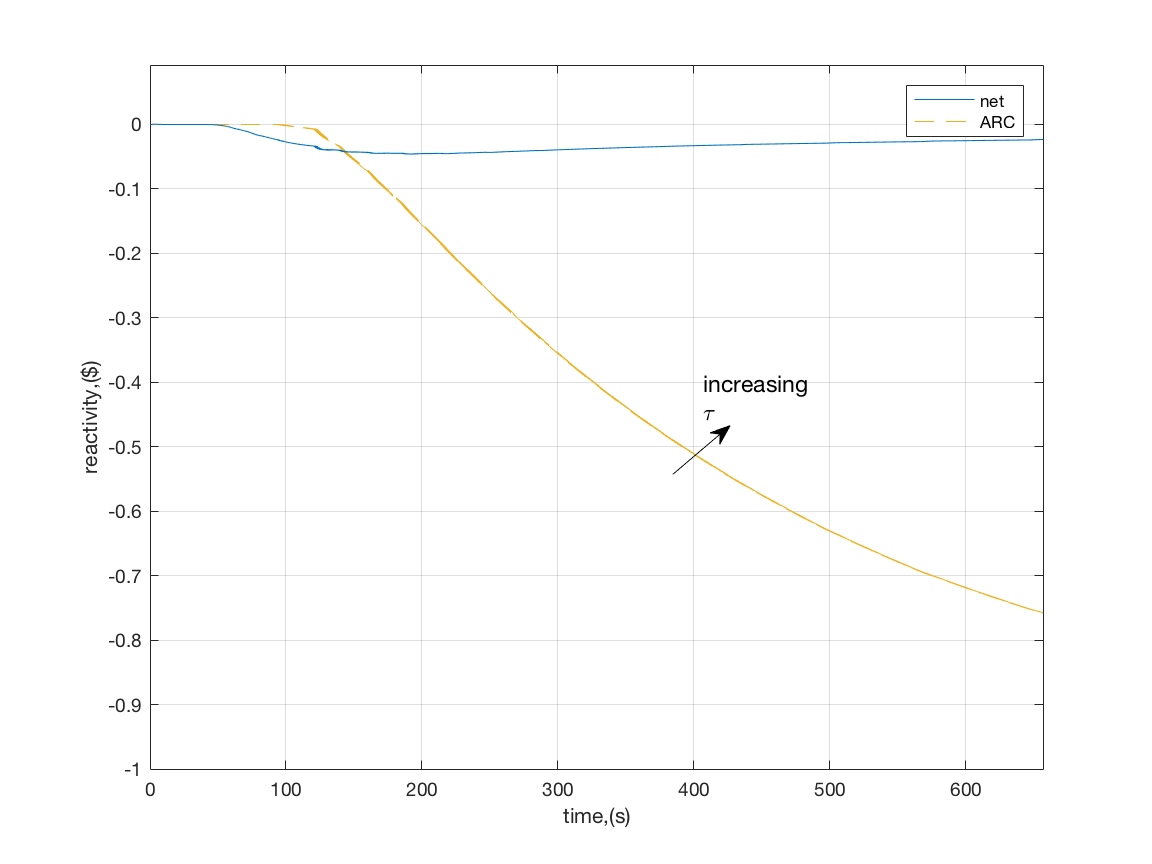
\includegraphics[width=10cm]{ULOHS_rho}
\centering
\caption{ARC and net reactivity in the oxide ABR ULOHS scenario for $\tau=[1.3, 1.8, 2.3, 2.8, 3.3, 3.8, 4.3, 4.8]$ s.}
\label{fig:ULOHS_rho}
\end{figure}

%%%%%%%%%%%%%%%%%%%%%%%%%%%%%%%%%%%%%%%%%%%%%%%%%%%%%%%%%%%%%%%%%%%%%%%
\section{UTOP}
Figure \ref{fig:UTOP_peak} shows the peak coolant temperatures with time of each UTOP simulation for all $\tau$ values on a single plot.
It is seen that the increasing $\tau$ value has a slight impact on the results and introduces some small oscillations, although the difference in temperatures between models is less than 1 C.
All oscillations induced by the increased $\tau$ are less than 1 C in magnitude and do not grow.
There is no clear trend with increasing $\tau$, and overall the results of the increased time lag are not safety significant. 
Figure \ref{fig:UTOP_rho} shows similar behavior for the reactivity during the transient.
Detailed evaluation of the ARC reactivity shows that small oscillations of less than \$0.01 are present with some values of $\tau$.
The small oscillations are triggered by the abrupt end to the rod withdrawal, which makes for a non-smooth reactivity component, and are present even in the case of very small $\tau$.
As with the temperature behavior, these oscillations persist for longer in some cases than others, but no trend exists where the oscillations continue to grow with further increasing $\tau$.
None of the examined $\tau$ values introduce oscillations into the UTOP response of any significance, and the maximum and asymptotic temperatures are unaffected.

\begin{figure}[h!]
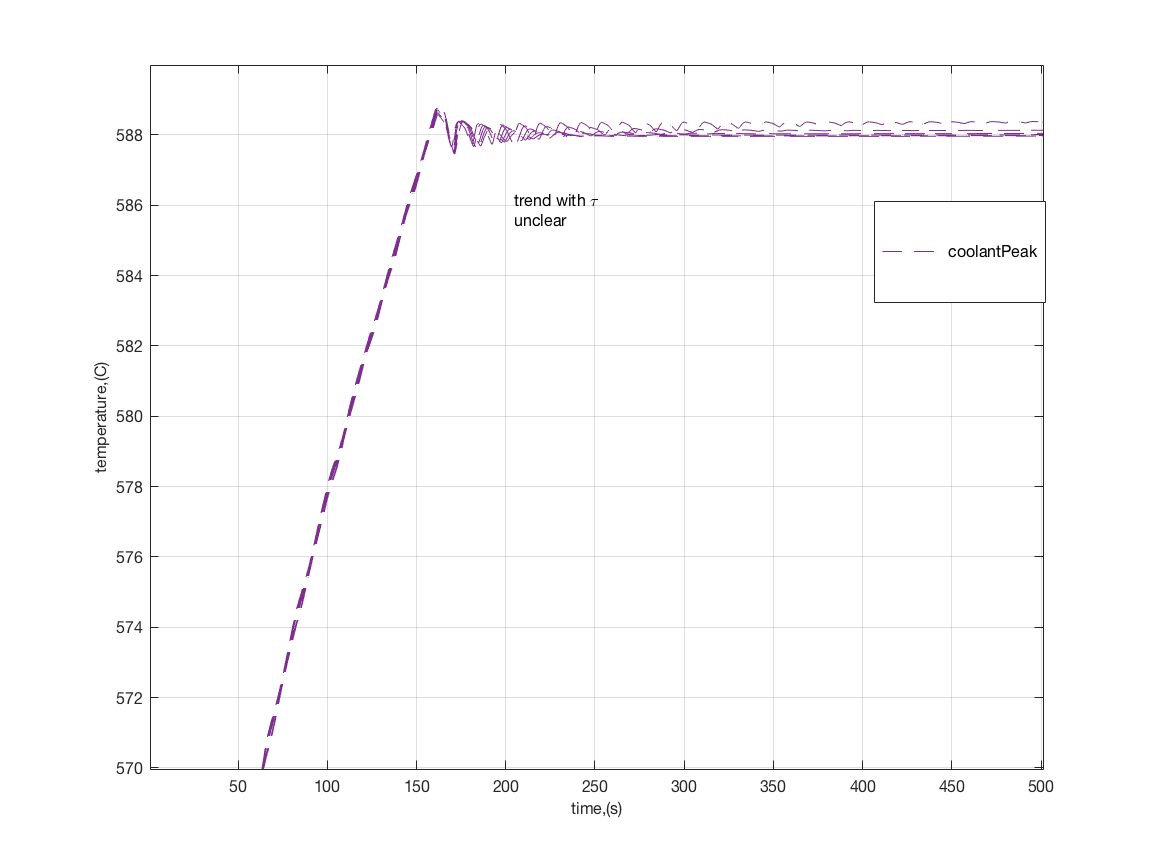
\includegraphics[width=10cm]{UTOP_peak}
\centering
\caption{Peak coolant temperature in the oxide ABR UTOP scenario for $\tau=[1.3, 1.8, 2.3, 2.8, 3.3, 3.8, 4.3, 4.8]$ s.}
\label{fig:UTOP_peak}
\end{figure}

\begin{figure}[h!]
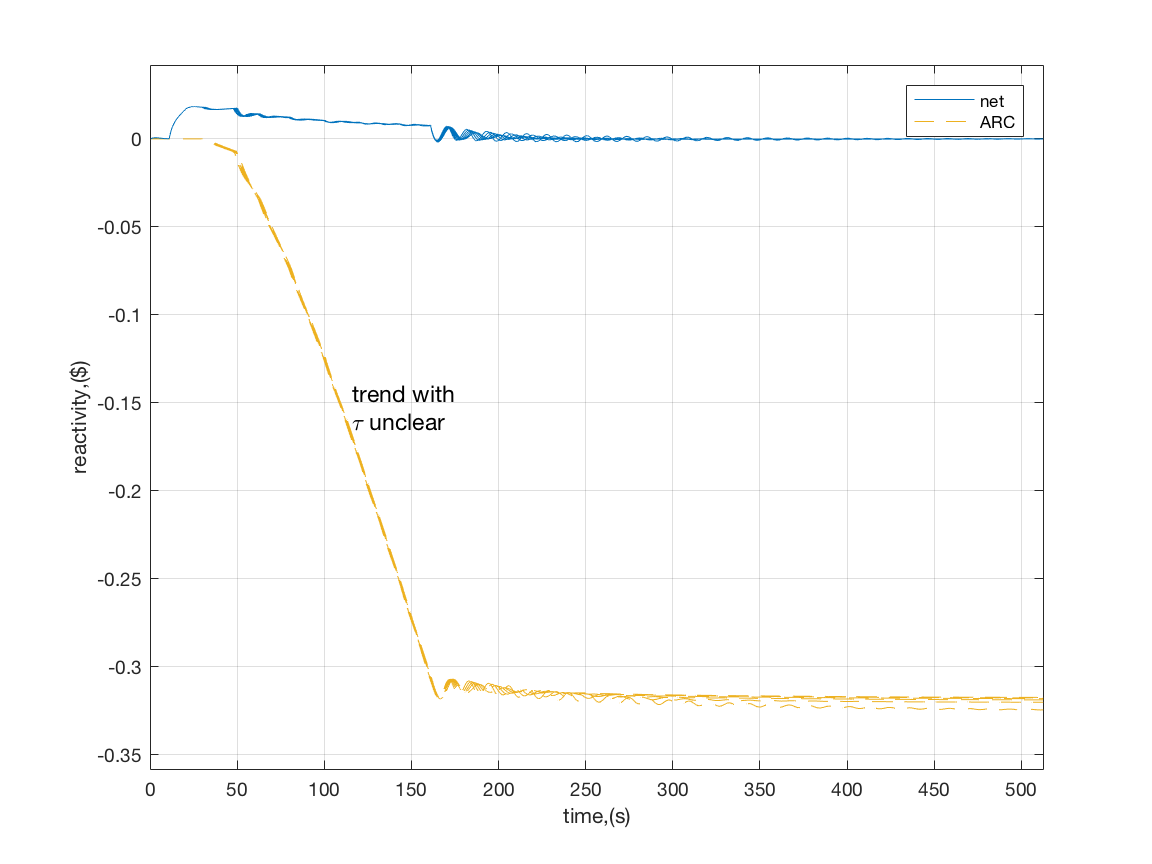
\includegraphics[width=10cm]{UTOP_rho}
\centering
\caption{ARC and net reactivity in the oxide ABR UTOP scenario for $\tau=[1.3, 1.8, 2.3, 2.8, 3.3, 3.8, 4.3, 4.8]$ s.}
\label{fig:UTOP_rho}
\end{figure}

%%%%%%%%%%%%%%%%%%%%%%%%%%%%%%%%%%%%%%%%%%%%%%%%%%%%%%%%%%%%%%%%%%%%%%%
\section{ULOF}
Figure \ref{fig:ULOF_peak} shows the peak coolant temperatures with time of each ULOF simulation for all $\tau$ values on a single plot over the first hour of the transient, while Figure \ref{fig:ULOF_peakShortTerm} shows the same curves zoomed in on the first 400 s to show in more detail the early phase oscillations.
For these simulations, the variable-lag-compensator in SAS was used along with the $\tau$ vs flow correlation developed by Qvist et. al \cite{1stARC_paper} to account for the reduced convective heat transfer from coolant to reservoir as the flow rate drops off.
As $\tau$ is increased, the small coolant peak temperature oscillations in the early phase of the transient (i.e. $<$ 500 s) remain stable, and none of the oscillations grow as the transient progresses. 
These oscillations become somewhat smaller and less pronounced as $\tau$ is increased.
In fact, examination of Figure \ref{fig:ULOF_rho} shows that the oscillations in both ARC and net reactivity are reduced as $\tau$ is increased.
The oscillations which are present due to the transition from forced to natural circulation at ~700 s are not impacted significantly by the increased $\tau$.
For further discussion of the cause and nature of these oscillations, see the detailed report by Keckler \cite{ULOF_oscillationsReport}.

Furthermore, as $\tau$ is increased, the peak coolant temperatures at later stages in the transient actually slightly decrease.
This is due to a cancelling effect within the reactivity feedbacks, which ends up dampening the net reactivity response and keeping the reactor state at a lower net reactivity for longer during the early transient phase, which later shows through as a slightly lower temperature at the asymptotic state.
This is depicted in Figure \ref{fig:ULOF_rho}.
The change with increasing $\tau$ is likely easier to see in the ULOF than the other transients due to the low flow conditions, which makes $\tau$ up to 5x larger than the nominal full-flow value. 
This very long time delay allows for more heat transfer from the oxide fuel to the coolant, which allows the coolant temperature to change more as the ARC reservoir is slowly heating up. 
This makes the different cases easier to differentiate from each other.

For the ULOF, a previous study by Qvist et al. has examined the sensitivity of the ARC response to the delay for temperature communication to the ARC upper reservoir \cite{ARC_Annals}.
Qvist et al. investigated the magnitude of oscillations induced by having an increasing mass of steel between the fuel and the ARC upper reservoir (effectively a longer time delay for heat transfer) and found that oscillations can be avoided for a particular $\tau$ if the equilibrium temperatures following the ULOF transient are allowed to be high enough.
Qvist et al. found that the equilibrium coolant temperatures should be ~725 C to avoid oscillations, no matter the $\tau$.
This study cannot be directly compared with the results of \cite{ARC_Annals}, however, due to the differing nature of the variations. 
Qvist et. al varies the time that it takes for the coolant temperature to be communicated from the top of the core to the axial level of the ARC reservoir, whereas this study varies the amount of time it takes for the coolant temperature to be communicated from the coolant \textit{already at the level of the reservoir} to the expander fluid within the upper reservoir.
A discussion of the difference between these two difference heat transfer delay mechanisms is given in \cite{ULOF_oscillationsReport}.

\begin{figure}[h!]
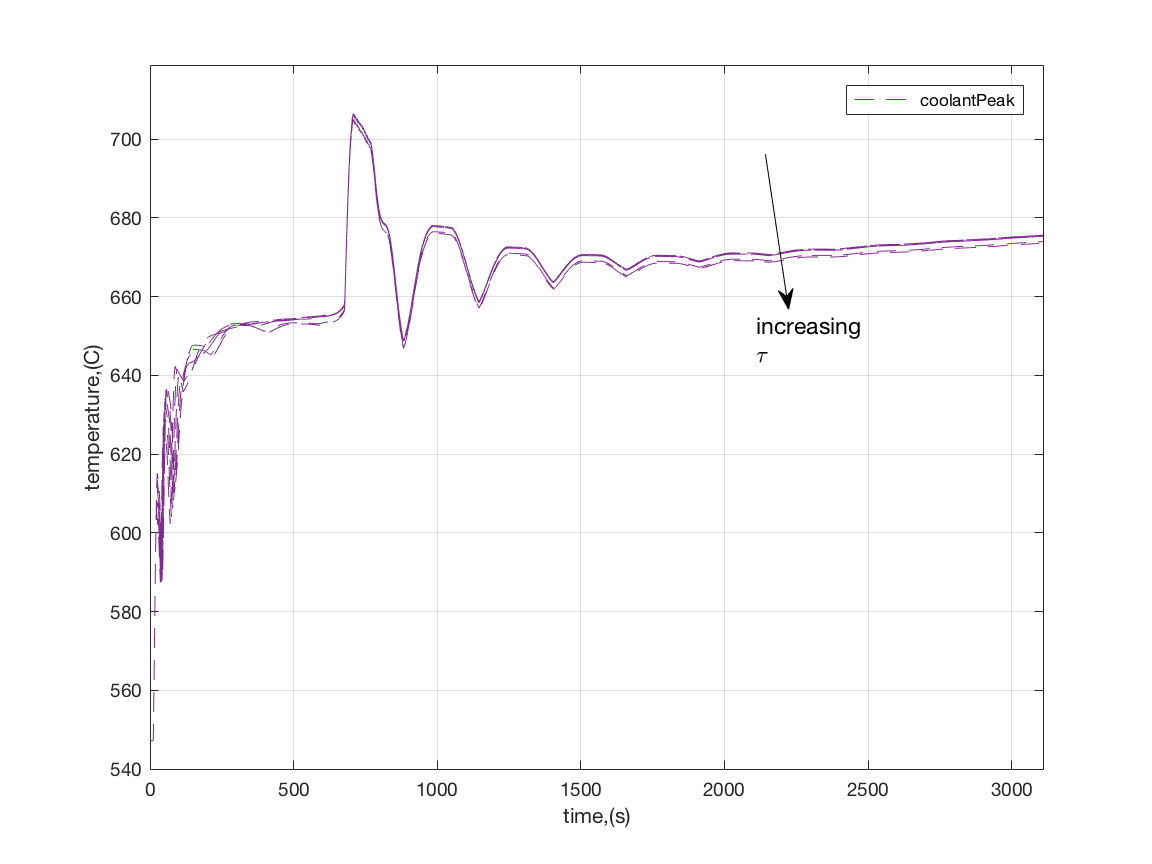
\includegraphics[width=10cm]{ULOF_peak}
\centering
\caption{Peak coolant temperature in the oxide ABR ULOF scenario for $\tau=[1.3, 1.8, 2.3, 2.8, 3.3, 3.8, 4.3, 4.8]$ s over the first hour of the transient.}
\label{fig:ULOF_peak}
\end{figure}

\begin{figure}[h!]
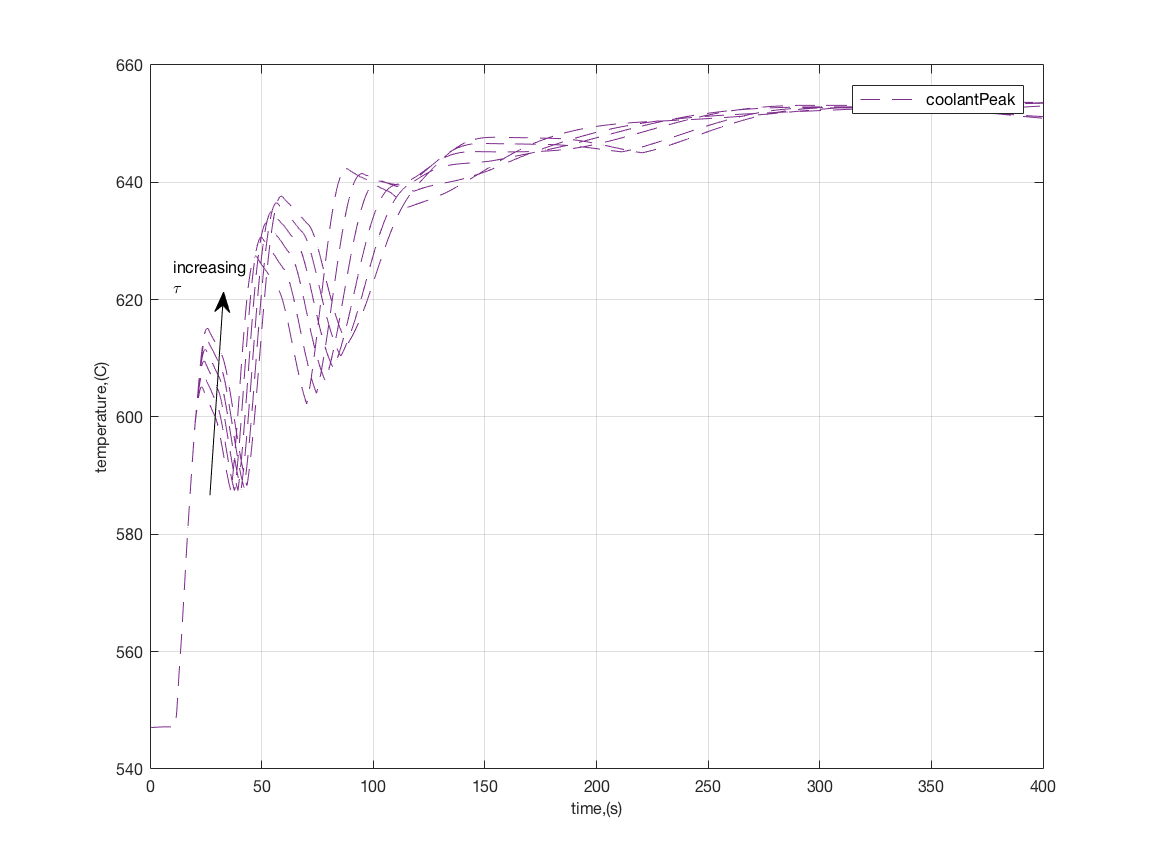
\includegraphics[width=10cm]{ULOF_peakShortTerm}
\centering
\caption{Peak coolant temperature in the oxide ABR ULOF scenario for $\tau=[1.3, 1.8, 2.3, 2.8, 3.3, 3.8, 4.3, 4.8]$ s in the first 400 s.}
\label{fig:ULOF_peakShortTerm}
\end{figure}

\begin{figure}[h!]
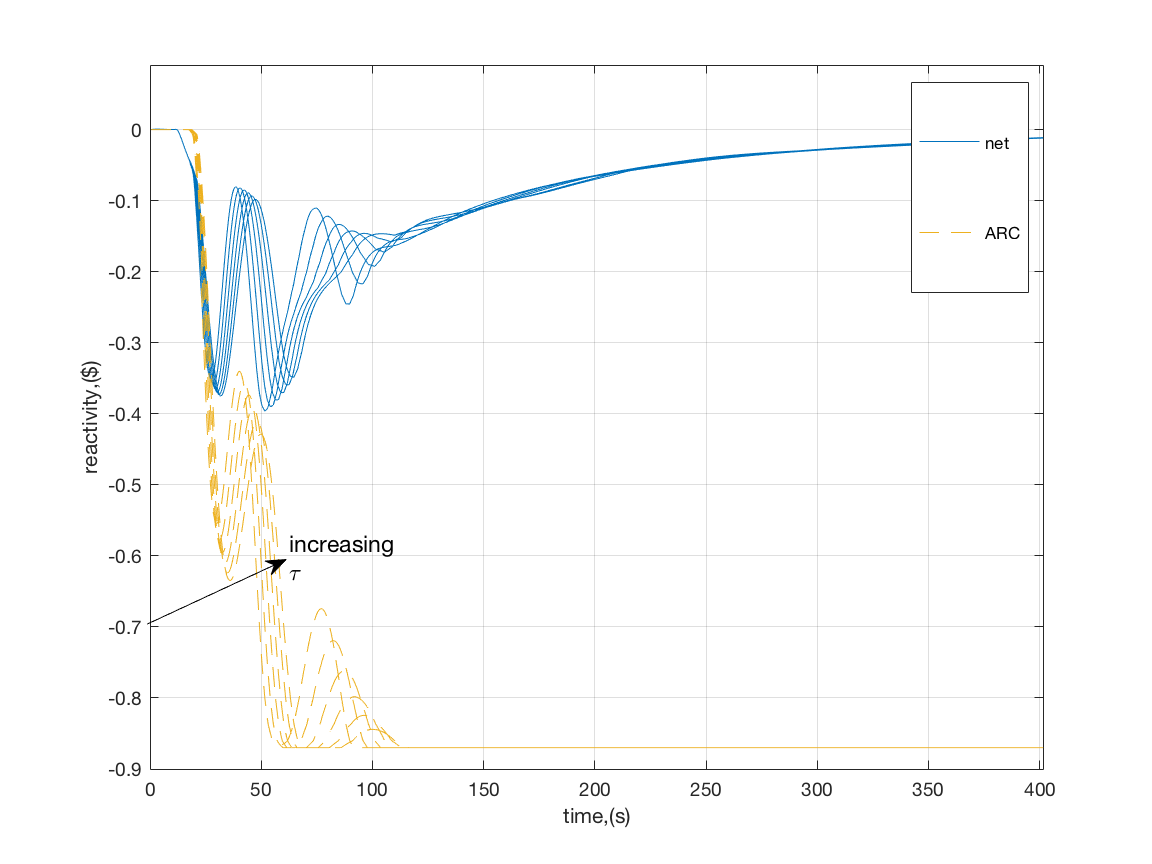
\includegraphics[width=10cm]{ULOF_rho}
\centering
\caption{ARC and net reactivity in the oxide ABR ULOF scenario for $\tau=[1.3, 1.8, 2.3, 2.8, 3.3, 3.8, 4.3, 4.8]$ s.}
\label{fig:ULOF_rho}
\end{figure}

%%%%%%%%%%%%%%%%%%%%%%%%%%%%%%%%%%%%%%%%%%%%%%%%%%%%%%%%%%%%%%%%%%%%%%%
\section{Conclusions}
This study examined the sensitivity of the transient ULOHS, UTOP, and ULOF behavior of the ARC-equipped oxide ABR with increasing heat transfer lag from the primary coolant to the ARC upper reservoir.
From the sensitivity study it is concluded that the response with the optimal ARC design chosen in \cite{2017ANSWinter_ARC} is not sensitive $\tau$.
Almost no difference is seen in the ULOHS with increasing $\tau$.
Very small differences are seen with increasing $\tau$ for the UTOP and ULOF scenarios, but these differences do not introduce any notable unstable behavior and are not detrimental to safety.
Therefore it is concluded that the physical design of the ARC upper reservoir should not be severely constrained to obtain a small $\tau$, and significant margin in the geometric design exists for minimizing the additional pressure drop and ensuring structural integrity.

%%%%%%%%%%%%%%%%%%%%%%%%%%%%%%%%%%%%%%%%%%%%%%%%%%%%%%%%%%%%%%%%%%%%%%%
\begin{thebibliography}{9}

\bibitem{2017ANSWinter_ARC}
C. Keckler, S. Qvist, T. Fanning, M. Fratoni, E. Greenspan. "SAS4A/SASSYS-1 Simulation of ARC System in Oxide ABR for Improved Safety Margin," ANS Winter Conference, Washington DC, 2017.

\bibitem{1stARC_paper}
S. Qvist, C. Hellesen, R. Thiele, A. Dubberley, M Gradecka, E. Greenspan. "Autonomous Reactivity Control (ARC) - Principles, geometry and design process," Nuclear Engineering and Design (2016).

\bibitem{ARC_Annals}
S. Qvist, C. Hellesen, M Gradecka, A Dubberley, T. Fanning, E. Greenspan, "Tailoring the response of Autonomous Reactivity Control (ARC) systems," Annals of Nuclear Energy (2016).

\bibitem{ULOF_oscillationsReport}
C. Keckler, "Oscillations in the Oxide-fuelled ABR ULOF with ARC System Implementation," Internal memo, 2017.

\end{thebibliography}

\end{document}